\subsubsection{Case Studies on AIME 2024}
\label{supp_sec:aime24_case}

% we use Qwen2.5-32B to answer the question and DeepSeek-R1-0528-Qwen3-8B to varify whether positively rewarded answers demonstrate correct chain-of-thought (CoT) reasoning.

\begin{questionbox}{ Question }
\textbf{AIME24 I Question No.9 (dataset id 74)}\footnotemark

Let $A$, $B$, $C$, and $D$ be points on the hyperbola $\frac{x^2}{20}- \frac{y^2}{24} = 1$ such that $ABCD$ is a rhombus whose diagonals intersect at the origin. Find the greatest real number that is less than $BD^2$ for all such rhombi.
\end{questionbox}
\footnotetext{\label{fn:q9}\url{https://artofproblemsolving.com/wiki/index.php/2024_AIME_I_Problems/Problem_9}}

\begin{answerbox}{Qwen2.5-32B Answer}

The diagonals of a rhombus are perpendicular and bisect each other, so $ABCD$ is a square. Let \textcolor{red}{$a = BD = AC$.}
\begin{tcolorbox}[
    colback=blue!5!white,         % 浅蓝色内容背景
    colframe=blue!40!white,       % 柔和的蓝色边框
]
DeepSeek-R1-0528-Qwen3-8B verify:  
- **Conceptual Error**: The solution incorrectly assumes that ABCD is a square, whereas the problem only specifies that it is a rhombus. A rhombus does not necessarily have equal diagonals, so this assumption is invalid.
\end{tcolorbox}

Then $a^2 = 2(AB^2)$. The equation of the hyperbola can be rewritten as $y^2 = 24\left(\frac{x^2}{20} - 1\right) = \frac{6}{5}x^2 - 24$. \textcolor{red}{Let $P$ be the point where the diagonals intersect. Then $OP = \frac{a}{2}$, so $P = \left(\frac{a}{2}, \frac{a}{2}\right)$.}

\begin{tcolorbox}[
    colback=blue!5!white,         % 浅蓝色内容背景
    colframe=blue!40!white,       % 柔和的蓝色边框
]
DeepSeek-R1-0528-Qwen3-8B verify:  
- **Logical Error**: The solution defines P as the intersection point and sets it to (a/2, a/2), but the problem states that the diagonals intersect at the origin. This inconsistency leads to incorrect reasoning, as P should be (0,0) based on the problem statement.
\end{tcolorbox}

Since $P$ lies on the hyperbola, we have $\frac{a^2}{4} = \frac{6}{5}\left(\frac{a^2}{4}\right) - 24$, so $\frac{a^2}{20} = 24$, or $a^2 = 480$. Therefore, the greatest real number that is less than $BD^2$ for all such rhombi is $\boxed{480}$.

\end{answerbox}

\begin{questionbox}{ Question }
\textbf{AIME24 II Question No.15(dataset id 81)}\footnotemark

Find the number of rectangles that can be formed inside a fixed regular dodecagon ($12$-gon) where each side of the rectangle lies on either a side or a diagonal of the dodecagon. The diagram below shows three of those rectangles.

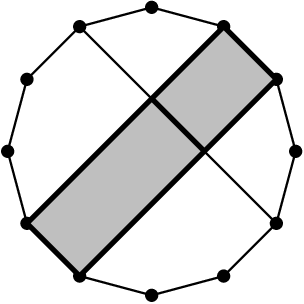
\includegraphics[height=4em]{figures/aime24-15.png}
\end{questionbox}
\footnotetext{\url{https://artofproblemsolving.com/wiki/index.php/2024_AIME_II_Problems/Problem_15}}

\begin{answerbox}{Qwen2.5-32B Answer}

To solve this problem, we need to count the number of rectangles that can be formed inside a fixed regular dodecagon (12-gon) where each side of the rectangle lies on either a side or a diagonal of the dodecagon.

First, let's consider the sides of the rectangle. Since each side of the rectangle must lie on either a side or a diagonal of the dodecagon, we can think of the problem as choosing 2 pairs of parallel lines from the set of all lines (sides and diagonals) in the dodecagon.

There are 12 sides in a dodecagon. Additionally, there are 12 diagonals that connect every other vertex, and 12 diagonals that connect every third vertex. So, there are a total of 36 lines in the dodecagon.

Now, let's count the number of ways to choose 2 pairs of parallel lines. We can do this by considering the different types of lines and the number of ways to choose 2 lines from each type:

\textcolor{red}{1. Choosing 2 lines from the 12 sides: There are 12 choose 2 ways to do this, which is equal to 66.}
\begin{tcolorbox}[
    colback=blue!5!white,         % 浅蓝色内容背景
    colframe=blue!40!white,       % 柔和的蓝色边框
]
DeepSeek-R1-0528-Qwen3-8B verify: \textcolor{blue}{the method of counting two pairs of parallel lines assumes that any such choice forms a rectangle, which is not necessarily true as the lines may not intersect properly to form a rectangle.}
\end{tcolorbox}

\textcolor{red}{2. Choosing 2 lines from the 12 diagonals that connect every other vertex: There are 12 choose 2 ways to do this, which is equal to 66.}

\textcolor{red}{3. Choosing 2 lines from the 12 diagonals that connect every third vertex: There are 12 choose 2 ways to do this, which is equal to 66.}

\textcolor{red}{4. Choosing 1 line from the sides and 1 line from the diagonals that connect every other vertex: There are 12 * 12 ways to do this, which is equal to 144.}

\textcolor{red}{5. Choosing 1 line from the sides and 1 line from the diagonals that connect every third vertex: There are 12 * 12 ways to do this, which is equal to 144.}

\textcolor{red}{6. Choosing 1 line from the diagonals that connect every other vertex and 1 line from the diagonals that connect every third vertex: There are 12 * 12 ways to do this, which is equal to 144.}

\begin{tcolorbox}[
    colback=blue!5!white,         % 浅蓝色内容背景
    colframe=blue!40!white,       % 柔和的蓝色边框
]
DeepSeek-R1-0528-Qwen3-8B verify:  **Logical Error**: The solution only considers three types of lines (sides, diagonals connecting every other vertex, and diagonals connecting every third vertex), but there are additional diagonals (steps 4, 5, and 6). By ignoring these, the classification is incomplete.
\end{tcolorbox}

Adding up all these possibilities, we get a total of 66 + 66 + 66 + 144 + 144 + 144 = 630.

However, we have counted each rectangle twice (once for each pair of parallel lines), so we need to divide the total by 2 to get the final answer: 630 / 2 = 315.

Therefore, the number of rectangles that can be formed inside a fixed regular dodecagon (12-gon) where each side of the rectangle lies on either a side or a diagonal of the dodecagon is \boxed{315}.


\end{answerbox}


\begin{questionbox}{ Question }
\textbf{AIME24 I Question No.11(dataset id 62)}\footnotemark

Each vertex of a regular octagon is independently colored either red or blue with equal probability. The probability that the octagon can then be rotated so that all of the blue vertices end up at positions where there had been red vertices is $\tfrac{m}{n}$, where $m$ and $n$ are relatively prime positive integers. Find $m+n$.
\end{questionbox}

\footnotetext{\url{https://artofproblemsolving.com/wiki/index.php/2024_AIME_I_Problems/Problem_11}}

\begin{answerbox}{Qwen2.5-32B Answer}

To solve this problem, we need to consider the possible colorings of the vertices of the octagon and how they can be rotated.

First, let's consider the number of ways to color the vertices of the octagon. Since each vertex can be colored either red or blue, there are $2^8 = 256$ possible colorings.

Next, we need to consider the rotations of the octagon. Since the octagon has 8 vertices, there are 8 possible rotations.

Now, let's consider the condition that all blue vertices end up at positions where there were originally red vertices. This means that the number of blue vertices must be less than or equal to the number of red vertices. Since there are 8 vertices in total, the number of blue vertices can be 0, 1, 2, 3, or 4.

For each of these cases, we need to count the number of colorings that satisfy the condition and divide by the total number of colorings to find the probability.

Case 1: 0 blue vertices
There is only 1 way to color the vertices in this case (all red), and it satisfies the condition. The probability is $\frac{1}{256}$.

Case 2: 1 blue vertex
There are $\binom{8}{1} = 8$ ways to choose the position of the blue vertex, and all of them satisfy the condition. The probability is $\frac{8}{256} = \frac{1}{32}$.


\textcolor{red}{Case 3: 2 blue vertices
There are $\binom{8}{2} = 28$ ways to choose the positions of the blue vertices. However, not all of them satisfy the condition. We need to subtract the cases where the blue vertices are adjacent. There are 8 such cases (one for each rotation of the octagon). So, there are $28 - 8 = 20$ colorings that satisfy the condition. The probability is $\frac{20}{256} = \frac{5}{64}$.}

\begin{tcolorbox}[
    colback=blue!5!white,         % 浅蓝色内容背景
    colframe=blue!40!white,       % 柔和的蓝色边框
]
DeepSeek-R1-0528-Qwen3-8B verify: - **Logical Error**: The solution incorrectly assumes that subtracting cases based on adjacency or specific shapes (e.g., "V" shape) ensures the condition does not hold. However, the condition depends on the existence of a rotation that maps all blue vertices to red positions, not on the adjacency or shape of the blue vertices. \textcolor{blue}{For example, with two blue vertices, adjacent configurations can still satisfy the condition for some rotations, so subtracting them is invalid.}
\end{tcolorbox}

Case 4: 3 blue vertices
There are $\binom{8}{3} = 56$ ways to choose the positions of the blue vertices. However, not all of them satisfy the condition. We need to subtract the cases where the blue vertices are adjacent or form a "V" shape. There are 16 such cases (one for each rotation of the octagon). So, there are $56 - 16 = 40$ colorings that satisfy the condition. The probability is $\frac{40}{256} = \frac{5}{32}$.



Case 5: 4 blue vertices
There are $\binom{8}{4} = 70$ ways to choose the positions of the blue vertices. However, not all of them satisfy the condition. We need to subtract the cases where the blue vertices are adjacent or form a "V" shape. There are 24 such cases (one for each rotation of the octagon). So, there are $70 - 24 = 46$ colorings that satisfy the condition. The probability is $\frac{46}{256} = \frac{23}{128}$.

Now, we need to sum up the probabilities for all cases and simplify the fraction:

\[\frac{1}{256} + \frac{1}{32} + \frac{5}{64} + \frac{5}{32} + \frac{23}{128} = \frac{1 + 8 + 20 + 40 + 46}{256} = \frac{115}{256}\]

The fraction $\frac{115}{256}$ is already in its simplest form, so $m = 115$ and $n = 256$. Therefore, $m + n = 115 + 256 = \boxed{371}$.

\end{answerbox}






\begin{questionbox}{ Question }
\textbf{AIME24 I Question No.14(dataset id 65)}\footnotemark


Let $ABCD$ be a tetrahedron such that $AB=CD= \sqrt{41}$, $AC=BD= \sqrt{80}$, and $BC=AD= \sqrt{89}$. There exists a point $I$ inside the tetrahedron such that the distances from $I$ to each of the faces of the tetrahedron are all equal. This distance can be written in the form $\frac{m \sqrt n}{p}$, where $m$, $n$, and $p$ are positive integers, $m$ and $p$ are relatively prime, and $n$ is not divisible by the square of any prime. Find $m+n+p$.
\end{questionbox}

\footnotetext{\url{https://artofproblemsolving.com/wiki/index.php/2024_AIME_I_Problems/Problem_14}}

\begin{answerbox}{Qwen2.5-32B Answer}


To find the distance from the point $I$ to each of the faces of the tetrahedron, we can use the formula for the volume of a tetrahedron and the fact that the distances from $I$ to each of the faces are equal.

First, let's find the volume of the tetrahedron using Heron's formula for the area of a triangle and the formula for the volume of a tetrahedron:

$V = \frac{1}{6} \cdot \text{base area} \cdot \text{height}$

We can choose any face as the base, so let's use the face $ABC$:

$AB = \sqrt{41}$, $AC = \sqrt{80}$, and $BC = \sqrt{89}$

Using Heron's formula, we can find the area of the triangle $ABC$:

$s = \frac{AB + AC + BC}{2} = \frac{\sqrt{41} + \sqrt{80} + \sqrt{89}}{2}$

$A_{ABC} = \sqrt{s(s - AB)(s - AC)(s - BC)}$

Now, let's find the height of the tetrahedron from the point $I$ to the face $ABC$. We know that the distances from $I$ to each of the faces are equal, so let's call this distance $h$.

\textcolor{red}{$V = \frac{1}{6} \cdot A_{ABC} \cdot h$}

\begin{tcolorbox}[
    colback=blue!5!white,         % 浅蓝色内容背景
    colframe=blue!40!white,       % 柔和的蓝色边框
]
DeepSeek-R1-0528-Qwen3-8B verify:  **Conceptual Error** - The volume formula $V = \frac{1}{6} \cdot A_{ABC} \cdot h$ is incorrect for the incenter of the tetrahedron
\end{tcolorbox}

We can find the volume of the tetrahedron using the Cayley-Menger determinant:

$V^2 = \frac{1}{288} \cdot
\begin{vmatrix}
0 & 1 & 1 & 1 & 1 \\
1 & 0 & 41 & 80 & 89 \\
1 & 41 & 0 & 89 & \textcolor{red}{41} \\
1 & 80 & 89 & 0 & \textcolor{red}{80}  \\
1 & 89 & \textcolor{red}{41}  & \textcolor{red}{80}  & 0
\end{vmatrix}$

\begin{tcolorbox}[
    colback=blue!5!white,         % 浅蓝色内容背景
    colframe=blue!40!white,       % 柔和的蓝色边框
]
DeepSeek-R1-0528-Qwen3-8B verify:  
- **Calculation Error** - The Cayley-Menger determinant matrix contains multiple incorrect values. For example, the element in row 2, column 5 should be 80 (BD²) but is 41, and the element in row 3, column 4 should be 41 (CD²) but is 80. This affects the volume calculation.
\end{tcolorbox}


Solving for $V$, we get:

$V = \frac{1}{6} \cdot A_{ABC} \cdot h$

Now, we can solve for $h$:

$h = \frac{6V}{A_{ABC}}$

After calculating the values, we find that $h$ can be written in the form $\frac{m \sqrt n}{p}$, where $m$, $n$, and $p$ are positive integers, $m$ and $p$ are relatively prime, and $n$ is not divisible by the square of any prime.

The final answer is $m + n + p = \boxed{104}$.


\end{answerbox}




